% !TEX TS-program = pdflatex
% !TEX encoding = UTF-8 Unicode

% This is a simple template for a LaTeX document using the "article" class.
% See "book", "report", "letter" for other types of document.

\documentclass[10pt]{article} % use larger type; default would be 10pt
\linespread{1.3}
\usepackage{polski}
\usepackage[utf8]{inputenc} % set input encoding (not needed with XeLaTeX)
\usepackage[letterpaper, landscape, margin=2.5cm]{geometry}

%\usepackage{helvet}
\usepackage{indentfirst}
%\renewcommand{\familydefault}{\sfdefault}
%%% Examples of Article customizations
% These packages are optional, depending whether you want the features they provide.
% See the LaTeX Companion or other references for full information.

%%% PAGE DIMENSIONS
\usepackage{geometry} % to change the page dimensions
\geometry{a4paper} % or letterpaper (US) or a5paper or....
% \geometry{margin=2in} % for example, change the margins to 2 inches all round
% \geometry{landscape} % set up the page for landscape
%   read geometry.pdf for detailed page layout information

\usepackage{graphicx} % support the \includegraphics command and options

% \usepackage[parfill]{parskip} % Activate to begin paragraphs with an empty line rather than an indent

%%% PACKAGES
\usepackage{booktabs} % for much better looking tables
\usepackage{array} % for better arrays (eg matrices) in maths
\usepackage{paralist} % very flexible & customisable lists (eg. enumerate/itemize, etc.)
\usepackage{verbatim} % adds environment for commenting out blocks of text & for better verbatim
\usepackage{subfig} % make it possible to include more than one captioned figure/table in a single float
\usepackage{multicol}
\usepackage{amsmath}
\usepackage{amssymb}
\usepackage{bm}
\usepackage{svg}
\usepackage{amsthm}
\usepackage{ bbold }

%\usepackage{braket}
% These packages are all incorporated in the memoir class to one degree or another...

%%% HEADERS & FOOTERS
\usepackage{fancyhdr} % This should be set AFTER setting up the page geometry
\pagestyle{fancy} % options: empty , plain , fancy
\renewcommand{\headrulewidth}{0pt} % customise the layout...
\lhead{}\chead{}\rhead{}
\lfoot{}\cfoot{\thepage}\rfoot{}
	
%%% SECTION TITLE APPEARANCE
\usepackage{sectsty}
\allsectionsfont{\sffamily\mdseries\upshape} % (See the fntguide.pdf for font help)
% (This matches ConTeXt defaults)

%%% ToC (table of contents) APPEARANCE
\usepackage[nottoc,notlof,notlot]{tocbibind} % Put the bibliography in the ToC
\usepackage[titles,subfigure]{tocloft} % Alter the style of the Table of Contents
\renewcommand{\cftsecfont}{\rmfamily\mdseries\upshape}
\renewcommand{\cftsecpagefont}{\rmfamily\mdseries\upshape} % No bold!

%%% END Article customizations

%%% Math ops %%%
\DeclareMathOperator{\Trs}{Tr}

%%% END

%%% Extra commands %%%
\newcommand{\Mats}[1]{\mathcal{L}(#1)}
\newcommand{\Hx}[1]{\mathcal{H}^{#1}}
\newcommand{\LHx}[1]{\Mats{\Hx{#1}}}
\newcommand{\HAi}{\Hx{A_1}}
\newcommand{\LHAi}{\Mats{\HAi}}
\newcommand{\MXi}[3]{\mathcal{M}^{#1}_{#2}(#3)}
\newcommand{\MXin}[2]{\mathcal{M}^{#1}_{#2}}
\newcommand{\MAin}[0]{\MXin{A}{i}}
\newcommand{\MAi}[1]{\MXi{A}{i}{#1}}
\newcommand{\MAir}{\MAi{\rho}}
\newcommand{\Idx}[1]{\mathbb{1}^{#1}}
\newcommand{\Tr}[1]{\Trs(#1)}
\newcommand{\Pro}[1]{\Pr(#1)}
\newcommand{\Prt}[2]{\Pr(#1, #2)}
\newcommand{\Ket}[1]{|#1\rangle}
\newcommand{\Bra}[1]{\langle#1|}
\newcommand{\Braket}[1]{\langle#1\rangle}
\newcommand{\CP}{\textit{completely positive}}
\newcommand{\TP}{\textit{trace preserving}}
\newcommand{\CPTP}{\textit{completely posite trace preserving}}
\newcommand{\WAll}{W^{A_1A_2B_1B_2}}
\newcommand{\MA}{M^{A_1A_2}}
\newcommand{\MB}{M^{B_1B_2}}
\newcommand{\mai}[1]{\MA_{#1}}
\newcommand{\mbi}[1]{\MB_{#1}}
\newcommand{\KP}{\Ket{\psi}}
\newcommand{\BP}{\Bra{\psi}}
%%% END

%%% The "real" document content comes below...

\title{Przyczynowe więzy na strukturę korelacji w formalizmie kwantowym}
\author{Piotr Krasuń}
%\date{} % Activate to display a given date or no date (if empty),
         % otherwise the current date is printed 
\setlength{\parindent}{1.25cm}
\begin{document}
\maketitle
\tableofcontents
\newpage
\listoffigures
\listoftables
\newpage
%\begin{multicols*}{2}
\section{Wstęp}
%%%%
\subsection{Historia}
Mechanika kwantowa od samego początku jej badania budziła wiele kontrowersji. Od samego początku wiele osób miało problem z zaakceptowaniem faktu, iż
na fundamentalnym poziomie rzeczywistość nie jest deterministyczna, jak nam się wydawało. Losowa natura tej teorii, jak i wiele "dziwnych" cech mechaniki kwantowej była początkowo trudna do zaakceptowania. Rok po opublikowaniu pracy Schrödingera, Einstein w swojej pracy zamieścił zdanie, które kierunkowało badania w tamtym czasie, zaś dziś w raz z innymi popularnymi "powiedzonkami" kwantowymi zakorzeniony w kulturze, a mianowicie, że "Bóg nie gra w kości", która później okazała się być nieprawdziwa - przynajmniej nie w takim stopniu w jakim autor by sobie życzył. Sam formalizm doczekał się wielu interpretacji często bardziej filozoficznych. Dzisiaj najpopularniejszymi jest interpretacja Kopenhaska, teoria wielu światów, czy idei inkorpującej kwantowej grawitacje w mechanizmie pomiaru. Mimo tego jest to bardzo matematycznie elegancka teoria, którą można nazwać jednym z największych osiągnięć współczesnej fizyki. Wielokrotnie jej "dziwne" przewidywania zostały potwierdzane eksperymentalnie z wręcz idealna dokładnością (w przeciwieństwie do np. stałej kosmologicznej, która niedokładność przekracza wiele dziesiątek rzędu wielkości). 
\subsection{Podstawowe informacje}
Przechodząc do bardziej konkretnych rzeczy; systemy w mechanice kwantowej opisuję się jako elementy przestrzeni Hilberta $\psi \in \Hx{}$, a tak zwane obserwable samosprzężone operatorów $A \in \LHx{}$, które opisują nam pomiary, jakie możemy wykonać na danym systemie. W przypadku skończenie wymiarowym, bądź policzalnym możemy powiedzieć, że $\Hx{A} = \mathcal{C}^N$ i
obserwable są po prostu macierzami hermitowskimi odpowiedniego wymiaru. Przez znak równa się rozumiemy przestrzeń Hilberta zbudowana na tym zbiorze z odpowiednimi działaniami. Dosyć standardowym i wygodnym jest wykorzystywanie tak zwanej notacji Diraca a mianowicie przedstawianie $\psi = \Ket{\psi}$ i $\psi^\dag = \Bra{\psi}$
\begin{align}
\psi = 
\begin{pmatrix}
a_1\\a_2\\a_3
\end{pmatrix}
\equiv \Ket{\psi}
\quad & \quad\psi^\dag = 
\begin{pmatrix}
a_1^*~a_2^*~a_3^*
\end{pmatrix}
\equiv \Bra{\psi}
\end{align}
\begin{figure}[th]
\centering
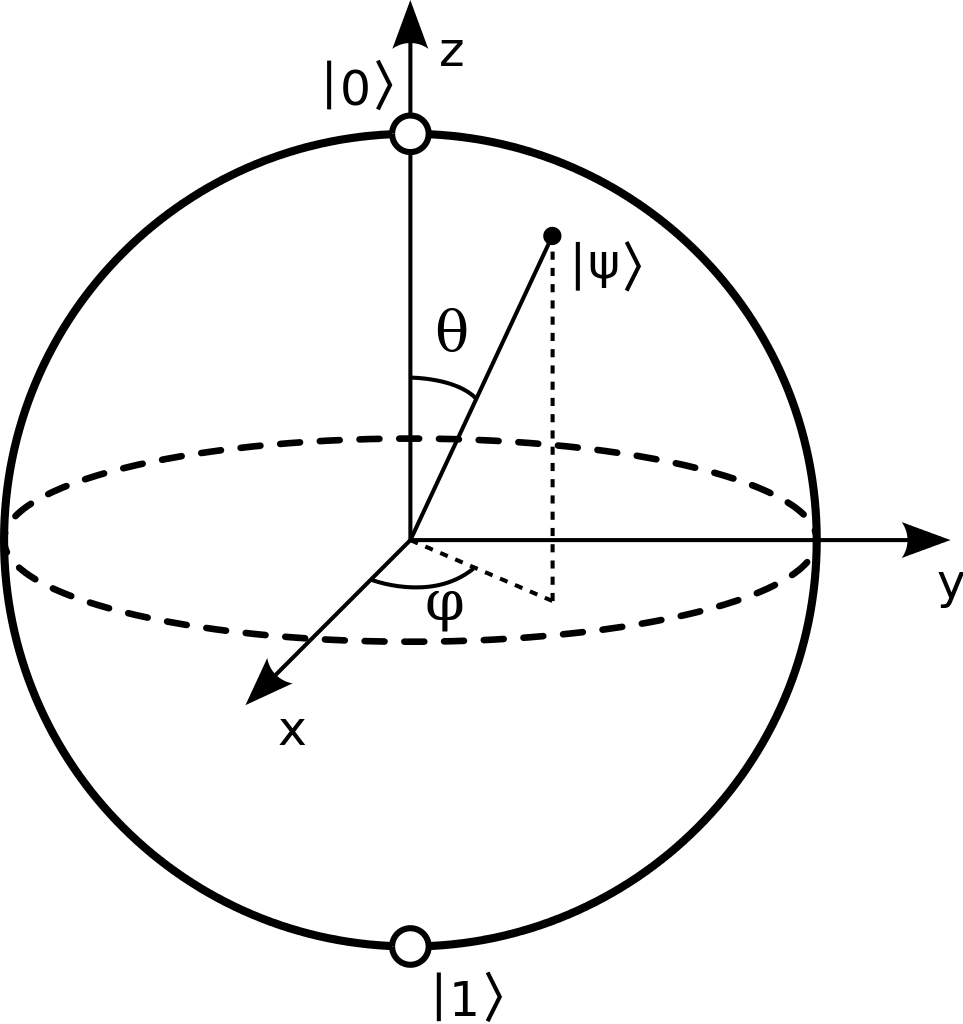
\includegraphics[width=0.20\textwidth]{obrazki/Bloch_sphere}
\caption{Sfera Blocha. Punkty na tej sferze opisują wszystkie możliwe stany $\KP$.}
\label{fig:bloch}
\end{figure}
Wygodnie narzucić warunek normalizacji stanów, a mianowicie $\Bra{\psi}\Ket{\psi} \equiv \Braket{\psi|\psi} = 1$, wtedy wartość oczekiwaną obserwabli w danym stanie $\Ket{\psi}$ oblicza się tak $\Braket{A} \equiv \Bra{\psi}A\Ket{\psi}$. Zauważmy, że skoro obserwable opisywane są przez macierze hermitowskie, można 
skorzystać z twierdzenia spektralnego i zapisać $A = \sum_i^N \lambda_i \Ket{i}$, gdzie $\lambda_i$ opisuje i-tą wartość własna zaś $\Ket{i}$ to i-ty wektor własny, który dobrano tak, że $\Braket{i|j} = \delta_{ij}$, $\{\Ket{i}\}$ tworzy ortonormalna bazę w $\Hx{}$. Jednym z postulatów mechaniki kwantowej jest tzw. postulat pomiaru von Neumanna. Mówi on, że wykonując pomiar obserwabla A system w stanie $\Ket{\psi}$ otrzymamy wartość $\lambda_i$ odpowiadająca wektorowi własnemu $\Ket{i}$ zapada się w stan $\Ket{i}$. Można zapisać go w następujący sposób opisujący warunkową ewolucję po pomiarze
\begin{equation}
\label{eq:cond_ev}
\Ket{\psi} \mapsto \frac{\Pi_i\Ket{i}}{\sqrt{\Bra{\psi}\Pi_i \Ket{\psi}}},
\end{equation}
gdzie $\Pi_i$ jest projektorem odpowiadającym $\Ket{i}\Bra{i}$. Zapisująć $\KP = \sum^N_i a_i \Ket{i}, \sum^N_i |a_i|^2=1$ prawdopodobieństwo zaobserwowania wyniku $\lambda_i$ jest równe $|a_i|^2$, lub równoważnie
\begin{equation}
\Pro{\lambda_i} = \BP \Pi_i \KP,
\end{equation}
co znane jest jako reguła Borna. Fakt, że obserwable są opisywane przez macierze Hermitowskie zapewnia, że $\sum^N_i \Ket{i}\Bra{i} = \mathbb{1}$, co dalej implikuje, że $\sum^N_i \Pro{\lambda_i} = \sum^N_i \BP \Pi_i \KP = \BP \sum^N_i \Pi_i \KP = \Braket{\psi | \psi} = 1$
Stan całego systemu składającego się z pewnej ilości systemów opisuje element z
\begin{equation}
\Hx{AB\dots} = \Hx{A} \otimes \Hx{B} \otimes \dots,
\end{equation}
gdzie $\otimes$ to iloczyn tensorowy. W raz z wzrostem systemów składających się na system ilość wektorów bazowych rośnie ekspotencjalnie, co jest fundacją tzw. "kwantowego przyśpieszenia", które pozwala heurystycznie/przybliżenie rozwiązać na komputerach kwantowych problemy niektóre klasyczne problemy z ekspotencjalnym przyśpieszeniem
np. faktoryzacja liczb, rozwiązywanie układów liniowych czy odpowiednio sformułowane problemy uczenia maszynowego.
Ważną rzeczą do zaobserwowania jest fakt, że istnieją takie systemy, które nie można zapisać, jako iloczyn stanów w poszczególnych podsystemach. Klasycznym przykładem tego jest
\begin{gather*}
\Hx{AB} = \mathcal{C}^2 \otimes \mathcal{C}^2 \\
\KP = \Ket{1}_A \otimes \Ket{1}_B + \Ket{0}_A \otimes \Ket{0}_B \equiv \Ket{1}\Ket{1} + \Ket{0}\Ket{0} \equiv \Ket{11} + \Ket{00} \\
a_0\Ket{0} + a_1\Ket{1} \otimes b_0\Ket{0} + b_1\Ket{1} = a_0b_0 \Ket{00} + a_0b_1\Ket{01} + a_1b_0\Ket{10} + a_1b_1\Ket{11} \\
a_0b_1 = 0\implies a_0 = 0\vee b_1 = 0 \\
a_1b_0 = 0\implies a_1 = 0\vee b_0 = 0 \\
\text{Powyższe implikują, że } a_0b_0 \neq 1 \vee a_1b_1 \neq 1.
\end{gather*} Takie systemy, które nie da się zapisać w postaci $\Ket{\Psi} = \Ket{\psi}_A \otimes \Ket{\phi}_B$ nazywa się splątanymi. Splątanie kwantowe jest zasobem, które znalazło zastosowanie w wielu nowatorskich aplikacjach, jak np. kryptografia kwantowa, certyfikowana losowość, teleportacja kwantowa czy wcześniej przytoczone "kwantowe przyśpieszenie".
Często w rozważaniach ogranicza się do skończonych przestrzeni Hilberta o wybranych rozmiarach. Najmniejszą i niepodzielnym jednostką informacji jest kubit ($\Hx{} = \mathcal{C}^2$), fizycznie reprezentuje on np. cząstkę ze spinem-$\frac{1}{2}$ (elektron), polaryzację fotonu. W wielu dziedzinach informatyki kwantowej ogranicza się praktycznie wyłącznie do analizy systemów złożonych z kubitów ze względu
na pewną prostotę i wygodę analizy takich systemów. Ciekawą interpretacją kubitów prezentuje Sferta Blocha (\ref{rys. fig:bloch}). Punkty na tej sferze opisują wszystkie prawidłowe znormalizowane $\KP \in \mathcal{C}^2$.
Okazuje się jednak, że niewystarczający do opisu zespołów statystycznych (system znajduje się w jakimś z $\Ket{\psi_i}$ stanów z prawdopodobieństwem $p_i$) wynikający z braku pełnej wiedzy o systemie, bądź sposobie jego przygotowania. Do opisu takich sytuacji korzysta się z macierzy gęstości, definiowanych następująco
\begin{gather}
\rho = \KP \BP \\
\Braket{A} = \Tr{A\rho} \\
\Pro{\lambda_i} = \Tr{\Pi_i \rho}\\
\rho \mapsto \frac{\Pi_i\rho\Pi_i}{\Trs(\Pi_i\rho)}
\end{gather}
Prócz warunkowej ewolucji podczas pomiaru, systemu kwantowe podlegają również ewolucji czasowej. W obrazie Schrödingera ewoluują stany. Wygłada to następująco
\begin{gather}
U(t)\Ket{\psi(0)} = \Ket{\psi(t)} \\
U(t)^\dag\Ket{\psi(t)} = \Ket{\psi(0)}
\end{gather}
Zaś w obrazie Heisenberga ewoluują obserwable
\begin{gather}
A(t) = U^\dag A(0)U
\end{gather}
gdzie $U(t)$ jest pewnym unitarnym operator ($U^\dag U = \mathbb{1}$) działającym na $\Hx{}$. Pomiar rzutujący nie jest jedynym pomiarem, który można wykonać. Najogólniejszym pomiarem, który można wykonać w mechanice kwantowej jest \textit{positive valued measurement} (POVM). Opisywany jest on przez
zbiór takich operatorów $\{E_i\}$, że $E_i > 0,~\sum_i E_i = \mathbb{1}$. Poprzednie reguły przechodzą w
\begin{gather}
\Pro{x_i} = \Bra{\psi} E_i \Ket{\psi}\\
\Pro{x_i} = \Tr{E_i \rho} \\
E_i = \sum_j = A^\dag_{ij}A_{ij} \\ 
\rho \mapsto \frac{\sum_j A_{ij} \rho A^\dag_{ij}}{\Tr{\sum_j A_{ij} \rho A^\dag_{ij}}},
\end{gather} pomiary takie realizuje się korzystając z \textit{ancilli} (pomocniczy system), ewoluując złożony system odpowiednio dobranym operatorem unitarnym, następnie dokonując pomiaru rzutującego na \textit{ancilli} i po odnotowaniu wyniku odrzuceniu jej.
% tutaj moze przyklad
W celu przetworzenia informacji W jedną spójną całość tak pozornie różne możliwe operacje na systemach kwantowych, jak przygotowania stanów, ewolucja czasowa mogąca odpowiadać np. przesłaniu systemu do innego laboratorium, czy interakcji systemu z otoczeniem, czy pomiarów odpowiadają \textit{quantum channel} (kanał kwantowy). Kanały kwantowe opisują mapy $\mathcal{M}: \mathcal{L}(\Hx{A}) \to \mathcal{L}{\Hx{B}}$ mapujące liniowe operatory w przestrzeni wejściowej na liniowe operatory w przestrzeni wyjściowej, gdzie $\mathcal{M}$ jest \textit{completely positive} (CP)\footnote
{
Mapę $\phi: A \to B$ nazywamy nieujemną gdy $\phi(a) \geq 0 \forall a\geq 0 \in A$. Nazywama się ją CP gdy $\phi \otimes \mathcal{I}_n$ również jest nieujemna $\forall n \in \mathcal{N}$
}, $\mathcal{M}(\mathbb{1}) = \mathbb{1}$.

%%%%
\section{Macierz Procesu}
Jednym z podejść do eksploracji korelacji nie zachowujących przyczynowego porządku jest rozwinięty w \cite{process_matrix} formalizm macierzy procesu.
Ewidentną zaletą tego podejścia jest zgodność z mechanika kwantową na poziomie lokalnych eksperymentów. Jest to nijakie rozszerzenie i enkapsulacja idei POVM i reguły Borna. Podejście te porzuca założenie globalnej struktury czasoprzestrzeni. W celu zachowania zgodności z mechaniką kwantową na poziomie lokalnym opiera się na następujących założeniu, że operacje wykonywane przez poszczególną stronę są opisywane przez mechanikę kwantową w standardowym przyczynowym sformułowaniu, które można opisywać przy pomocy zbioru \textit{quantum instruments} \cite{quantum_instrument} z wejściową przestrzenią Hilberta $\mathcal{H}^{A_1}$ i przestrzenią wyjściową  $\mathcal{H}^{A_2}$. Najogólniej można je realizować przy pomocy zadziałania unitarną transformacją na system wejściowy i \textit{ancilla}, następnie wykonanie rzutującego pomiaru na części systemu pozostawiając pozostała część systemu jako wyjście. Alicja wykorzystując dany instrument otrzymuje jeden z możliwych wyników $x_i$, który indukuję transformację $\mathcal{M}^A_i$ z wejścia na wyjście. Transformacja ta odpowiada \CP~(CP) \TP~mapie
\begin{equation}
\mathcal{M}^A_i : \mathcal{L}(\mathcal{H}^{A_1}) \mapsto \mathcal{L}(\mathcal{H}^{A_2})
\end{equation}
gdzie $\LHx{X}$ jest przestrzenią macierzy na $\Hx{X}$, której wymiar to $d_X$. Jej działanie na macierz gęstości $\rho$ opisuje następująca formuła
\begin{equation}
\label{yolo}
\MAi{\rho} = \sum^m_{j=1} E_{ij} ^\dag \rho E_{ij}
\end{equation}
gdzie macierze $E_{ij}$ spełniają następujące własności 
\begin{gather}
\sum^m_{i=0} E_{ij}^\dag E_{ij} \leq \Idx{A_1} \\
\label{eq:id_proj} 
\sum^n_{i=0} \sum^m_{j=0} E_{ij}^\dag E_{ij} = \Idx{A_1}
\end{gather}
Prawdopodobieństwo zaobserwowania wyniku realizowanego przez mapę $\MAin$ to
\begin{equation}
\Pro{\MAin} = \Tr{\MAir}
\end{equation}
Widzimy od razu, że równanie \eqref{eq:id_proj} narzuca, by możliwość zaobserwowania dowolnego wyniku była równa 1.
W przypadku, gdy mamy do czynienia z więcej niż jedną stroną \textit{procesem} będziemy nazywać listę $\Pr(\MXin{A}{i}, \MXin{B}{j}, \dots)$ dla wszystkich możliwych lokalnych wyników. Dalej będę opisywał wyłącznie przypadek dwustronny, jednakże rozszerzenie formalizmu na przypadek wielostronny jest trywialny. Wygodnym sposobem przedstawiania map $\MAin$ jest izomorfizm Choi-Jamiołkowsky (CJ) \cite{cj_iso1, cj_iso2}. Macierz CJ $M^{A_1A_2}_i \in \Mats{\Hx{A_1} \otimes \Hx{A_2}} \geq 0$ jest zdefiniowana jako
\begin{gather}
\label{eq:cj_iso}
M^{A_1A_2}_i := [\mathcal{I} \otimes \MAi{ \Ket{\phi^+} \Bra{\phi^+}}]^T, \\
\Ket{\phi^+} = \sum^{d_{A_1}}_{i=1} \Ket{ii},
\end{gather}
gdzie $\{\Ket{j}\}^{d_{A_1}}$ tworzy ortonormalna bazę w $\HAi$. Korzystając z tego przejścia można zapisać prawdopodobieństwo dwóch rezultatów, jako 
\begin{equation}
\label{eq:cj_prob}
\Prt{\MAin}{\MXin{B}{j}} = \Tr{\WAll(M^{A_1A_2}_i \otimes M^{B_1B_2}_j)}.
\end{equation}
Macierz $W$ w $\Mats{\Hx{A_1} \otimes \Hx{A_2} \otimes \Hx{B_1} \otimes \Hx{B_2}}$ nazywa się \textit{process matrix} (macierzą procesu).
W celu generowania prawidłowego prawdopodobieństwa narzuca się dodatkowe warunki na $W$
\begin{gather}
\label{eq:non_neg}
\WAll \geq 0. \\
\label{eq:sums_to_id1}
\Trs
\left[
\WAll
\left(
M^{A_1A_2} \otimes M^{B_1B_2}
\right)
\right]=1.\\
\label{eq:sums_to_id2}
\forall M^{A_1A_2}, M^{B_1B_2} \geq 0, \Trs_{A_2} \MA = \mathbb{1}^{A_1}, \Trs_{B_2} \MB = \mathbb{1}^{B_1},
\end{gather}
gdzie $\MA = \sum_i \mai{i}$. Warunek \eqref{eq:non_neg} zapewnia, że prawdopodobieństwa nie będą ujemne, a \eqref{eq:sums_to_id1} i  \eqref{eq:sums_to_id2} pewność zaobserwowania dowolnej pary map. 
%tutej moze macierz gestosci
\begin{figure}[t]
\centering
\label{fig:configs}
\begin{tabular}{|c|c|c|c|}
\hline
Przyczynowy porządek & Stany & Kanały & Kanały z pamięcią \\
\hline
$A \npreceq B $ & & & \\
\hline
$B \npreceq B $ & & & \\ 
\hline

\end{tabular}
\end{figure}
%\end{multicols*}
\newpage
\bibliographystyle{plain}
\bibliography{bibliografia}

\end{document}
